\chapter{厄米可观测量、自旋与概率规则}

\lectureoverview{量子力学是一套关于概率的演算。要在不把理解替换为口号的情况下使用它，我们需要一条紧凑的数学链条：复相位、归一化态、厄米可观测量、本征值与本征向量、正交性，以及玻恩规则。随后，三个泡利矩阵把这条链条转化为关于电子自旋的具体预言。}

\section{复数的极坐标形式}

首先消除一个小的代数摩擦来源。复数
\begin{equation}
  z=x+iy
\end{equation}
是复平面上的一个点，其中\(x\)位于实轴上，\(y\)位于虚轴上。若该点具有极坐标\((r,\theta)\)，则
\begin{equation}
  x=r\cos\theta,
  \qquad
  y=r\sin\theta,
\end{equation}
因此
\begin{equation}
  z=r(\cos\theta+i\sin\theta)=re^{i\theta}.
  \label{eq:l03-polar-form}
\end{equation}
欧拉的记号很有用，因为角度加法公式变成了指数律
\begin{equation}
  e^{i\theta}e^{i\phi}
  =e^{i(\theta+\phi)}.
  \label{eq:l03-phase-product}
\end{equation}
事实上，将两个三角形式相乘得到
\begin{align}
& (\cos\theta+i\sin\theta)(\cos\phi+i\sin\phi)
\notag\\
&\qquad=\cos(\theta+\phi)+i\sin(\theta+\phi).
\end{align}
熟悉的求和公式全都包含在这一个乘法之中。

复共轭将点关于实轴反射：
\begin{equation}
  z^*=x-iy,
  \qquad
  (e^{i\theta})^*=e^{-i\theta}.
\end{equation}
因此，
\begin{equation}
  e^{i\theta}e^{-i\theta}=1.
\end{equation}
形如\(e^{i\theta}\)的数位于单位圆上，称为\emph{纯相位}。每个非零复数都是一个正模长乘以一个纯相位：
\begin{equation}
  z=|z|e^{i\theta},
  \qquad
  |z|^2=z^*z=x^2+y^2.
  \label{eq:l03-modulus-phase}
\end{equation}

\begin{classroomqa}
\lecturetimestamp{00:06:36}
\audiencequestion{把\(\theta\)变为\(-\theta\)是否对应于复平面中旋转方向的反转？}
\lecturerresponse{是的。正相位角与负相位角以相反的方向描绘单位圆。复共轭把\(e^{i\theta}\)变为\(e^{-i\theta}\)，即反射后的点，也是相位的逆。}
\end{classroomqa}

这就是今天所需的全部复数跑道：模长、相位、共轭与单位圆。

\section{量子力学作为概率演算}

现在我们转向公设。一个物理系统被制备在某个\emph{态}中；一次测量询问某个\emph{可观测量}的值；量子力学为可能的答案提供概率。

态是复向量空间中的向量。对于一个二能级自旋系统，
\begin{equation}
  \ket\psi=\alpha\ket{u}+\beta\ket{d},
  \qquad
  \ket{u}=\begin{pmatrix}1\\0\end{pmatrix},
  \qquad
  \ket{d}=\begin{pmatrix}0\\1\end{pmatrix}.
  \label{eq:l03-two-level-state}
\end{equation}
系数决定上/下概率，
\begin{equation}
  P(u)=|\alpha|^2,
  \qquad
  P(d)=|\beta|^2,
\end{equation}
因此态必须归一化：
\begin{equation}
  \braket{\psi}{\psi}
  =|\alpha|^2+|\beta|^2
  =1.
  \label{eq:l03-state-normalization}
\end{equation}
这里的维数指的是态空间中独立备选方案的数目，而不是普通空间的维数。一个具有三个互斥基态的系统将使用三个正交归一列和三个振幅。

概率并不能完全决定振幅。乘以一个纯相位不改变模长：
\begin{equation}
  |e^{i\theta}\alpha|^2=|\alpha|^2.
\end{equation}
因此，振幅包含的信息超出了针对这一个基的概率。当考虑不同的测量以及稍后的时间演化时，它的作用将变得可见。

基态是正交归一的：
\begin{equation}
  \braket{u}{u}=\braket{d}{d}=1,
  \qquad
  \braket{u}{d}=\braket{d}{u}=0.
\end{equation}
它们的正交性属于态的复空间。此时还不能把它与普通三维空间中成直角的两支箭头相混淆；这一区分将在本讲接近末尾时变得具有决定性。

\section{为什么可观测量是厄米的}

实验结果可以记录为实数。为了方便，我们可以把两个实数打包成一个复数，但指针读数本身总是可以分离为实量。在有限维中，量子可观测量由一类特殊的线性算子表示：厄米矩阵。

为了定义它们，首先通过交换行与列来转置一个矩阵：
\begin{equation}
  (M^T)_{ij}=M_{ji}.
  \label{eq:l03-transpose}
\end{equation}
满足\(M^T=M\)的实矩阵是对称的。对于复矩阵，相应的操作是厄米共轭，
\begin{equation}
  M^\dagger=(M^T)^*,
  \qquad
  (M^\dagger)_{ij}=M_{ji}^*.
  \label{eq:l03-dagger}
\end{equation}

\begin{figure}[htbp]
\centering
\includegraphics[width=0.88\linewidth]{lecture_03_figure_02.png}
\caption{转置、对称以及向厄米共轭的过渡共享同一个黑板布局。}
\lectureframe{00:23:06}
\end{figure}

\begin{definition}
矩阵 \(M\) 是 \emph{Hermitian} 的，如果
\begin{equation}
  M^\dagger=M,
  \qquad\text{equivalently}\qquad
  M_{ij}=M_{ji}^*.
  \label{eq:l03-hermitian}
\end{equation}
\end{definition}

对角元是实数，因为\(M_{ii}=M_{ii}^*\)。关于对角线反射的非对角元是共轭对。因此，一般的二乘二形式为
\begin{equation}
  M=
  \begin{pmatrix}
    a&z\\
    z^*&b
  \end{pmatrix},
  \qquad a,b\in\mathbb R.
  \label{eq:l03-hermitian-two}
\end{equation}
厄米性是实性条件的矩阵类比；它并不要求每个元素分别都是实数。

第一个回报来自两个基本的共轭恒等式：
\begin{equation}
  \braket{B}{A}=\braket{A}{B}^*,
  \label{eq:l03-inner-conjugation}
\end{equation}
以及，对任意\(M\)，
\begin{equation}
  \bra B M\ket A
  =
  \bigl(\bra A M^\dagger\ket B\bigr)^*.
  \label{eq:l03-matrix-element-conjugation}
\end{equation}
表达式\(\bra B M\ket A\)是一个数，即\(M\)的\(BA\)矩阵元。若\(M\)是厄米的且\(B=A\)，则
\begin{equation}
  \bra A M\ket A
  =
  \bigl(\bra A M\ket A\bigr)^*.
\end{equation}
因此它是实数。

\begin{proposition}
对每个厄米\(M\)，期望值
\begin{equation}
  \expect{M}_A=\bra A M\ket A
  \label{eq:l03-expectation}
\end{equation}
在每个归一化态\(\ket A\)中都是实数。
\end{proposition}

期望值的概率含义还有待进一步展开，但它的实在性已经解释了为什么厄米算符是观测量的自然候选者。

\begin{classroomqa}
\lecturetimestamp{00:33:22}
\audiencequestion{平均值所用的尖括号记号是否来自 bra--ket 记号？}
\lecturerresponse{是的。狄拉克的括号记号提供的正是同样的括号。在 \(\bra A M\ket A\) 中，算符被夹在代表该态的 bra 与 ket 之间，所得结果就是期望值。}
\end{classroomqa}

\begin{classroomqa}
\lecturetimestamp{00:34:31}
\audiencequestion{一个物理量本身能否具有虚数的测量值？如果测量结果都是实数，量子力学中为什么还需要复数？}
\lecturerresponse{一组测量结果总可以记录为实数，即使我们选择把一对数打包成一个复数。更尖锐的问题是，理论为什么会被驱使采用复振幅。先把这个问题搁置：答案与可逆的时间演化有关，而时间演化尚未引入。把理论限制在实向量上会失去重要的可能性。}
\end{classroomqa}

数学并非装饰。没有数学，纠缠可以被说得神秘莫测，却始终得不到定义。我们继续在最简单的设定中进行，即一个二能级系统，以便日后能够诚实地把两个这样的系统组合起来。

\section{本征值就是可能的测量结果}

\begin{definition}
若非零向量 \(\ket a\) 是 \(M\) 的本征向量，本征值为 \(\lambda_a\)，则
\begin{equation}
  M\ket a=\lambda_a\ket a.
  \label{eq:l03-eigenvalue-equation}
\end{equation}
\end{definition}
矩阵可以改变该向量的长度或相位，但不会把它变成态空间中的另一个方向。

对于厄米矩阵，本征值是实数。将方程~\eqref{eq:l03-eigenvalue-equation}左乘 \(\bra a\)，得到
\begin{equation}
  \bra a M\ket a
  =\lambda_a\braket{a}{a}.
\end{equation}
由厄米性，左边为实数，而右边的范数为实数且为正。因此
\begin{equation}
  \lambda_a
  =
  \frac{\bra a M\ket a}{\braket{a}{a}}
  \in\mathbb R.
  \label{eq:l03-real-eigenvalue}
\end{equation}

现在给出物理陈述：当 \(M\) 代表一个可观测量时，它的本征值就是对 \(M\) 进行测量所能返回的值。属于 \(\lambda_a\) 的本征向量是这样一种态：在该态中，该值以确定性出现。

最简单的例子是对角矩阵：
\begin{equation}
  M=
  \begin{pmatrix}
    m_{11}&0\\
    0&m_{22}
  \end{pmatrix}.
\end{equation}

\begin{figure}[htbp]
\centering
\includegraphics[width=0.72\linewidth]{lecture_03_figure_03.png}
\caption{抽象的本征值方程被置于第一个对角例子之上。}
\lectureframe{00:44:04}
\end{figure}

直接相乘得到
\begin{align}
  M\begin{pmatrix}1\\0\end{pmatrix}
  &=m_{11}\begin{pmatrix}1\\0\end{pmatrix},
  \notag\\
  M\begin{pmatrix}0\\1\end{pmatrix}
  &=m_{22}\begin{pmatrix}0\\1\end{pmatrix}.
  \label{eq:l03-diagonal-eigenvectors}
\end{align}

\begin{figure}[htbp]
\centering
\includegraphics[width=0.72\linewidth]{lecture_03_figure_04.png}
\caption{下基向量返回时乘以较低的对角元。}
\lectureframe{00:45:58}
\end{figure}

对于更大的对角矩阵，同样的规则成立：其对角元是本征值，其标准的 one-hot 列向量是本征向量。

\section{三个自旋矩阵}

对于沿第三轴方向的电子自旋，取
\begin{equation}
  \sigma_3=
  \begin{pmatrix}
    1&0\\
    0&-1
  \end{pmatrix}.
\end{equation}
它的本征态是 \(\ket u=(1,0)^T\)，本征值为 \(+1\)，以及 \(\ket d=(0,1)^T\)，本征值为 \(-1\)。因此，探测器可能给出的两个值就是这两个本征值。

第一轴方向的自旋矩阵为
\begin{equation}
  \sigma_1=
  \begin{pmatrix}
    0&1\\
    1&0
  \end{pmatrix}.
\end{equation}
它的候选本征向量先不归一化地写出，因为本征向量乘以任意非零标量后仍是本征向量。然而，物理态必须归一化：
\begin{align}
  \ket{x+}
  &=\frac{1}{\sqrt2}\begin{pmatrix}1\\1\end{pmatrix},
  &
  \sigma_1\ket{x+}&=+\ket{x+},
  \notag\\
  \ket{x-}
  &=\frac{1}{\sqrt2}\begin{pmatrix}1\\-1\end{pmatrix},
  &
  \sigma_1\ket{x-}&=-\ket{x-}.
  \label{eq:l03-sigma-one-eigenvectors}
\end{align}

\begin{figure}[htbp]
\centering
\includegraphics[width=0.72\linewidth]{lecture_03_figure_05.png}
\caption{非对角矩阵与等权候选向量出现在乘积完成之前。}
\lectureframe{00:50:29}
\end{figure}

\begin{classroomqa}
\lecturetimestamp{00:56:45}
\audiencequestion{能否不从代数求解，而是从几何上看出 \(\sigma_1\) 的本征向量？}
\lecturerresponse{在实二分量图像中，\(\sigma_1\) 交换基方向 \(E_1\) 与 \(E_2\)。对角方向 \((1,1)^T\) 保持不变，而另一条对角线 \((1,-1)^T\) 则反向。因此它们是本征向量，本征值分别为 \(+1\) 与 \(-1\)。这是分量空间中的一幅图像，尚不是关于物理自旋指针的陈述。}
\end{classroomqa}

剩下的矩阵是
\begin{equation}
  \sigma_2=
  \begin{pmatrix}
    0&-i\\
    i&0
  \end{pmatrix},
\end{equation}
其归一化本征向量为
\begin{equation}
  \ket{y+}=\frac{1}{\sqrt2}\begin{pmatrix}1\\i\end{pmatrix},
  \qquad
  \ket{y-}=\frac{1}{\sqrt2}\begin{pmatrix}1\\-i\end{pmatrix}.
  \label{eq:l03-sigma-two-eigenvectors}
\end{equation}
它们的本征值同样是 \(+1\) 与 \(-1\)。

这三个矩阵的平方都等于单位矩阵：
\begin{equation}
  \sigma_1^2=\sigma_2^2=\sigma_3^2=I.
  \label{eq:l03-pauli-squares}
\end{equation}
若 \(\sigma_i\ket a=\lambda\ket a\)，则把 \(\sigma_i\) 作用两次得到 \(\lambda^2=1\)，所以 \(\lambda=\pm1\)。相同的谱是第一个迹象，表明这些矩阵代表沿等价空间轴方向的自旋分量。

\section{不同的结果要求正交的态}

在证明下一定理之前，先说明它的含义。如果某个可观测量在两个态中给出两个不同的确定答案，那么对该可观测量的测量就能完美地区分这两个态。量子力学把这种完美可区分性表述为正交性。

\begin{theorem}
设 \(M\) 为厄米算符，且
\begin{equation}
  M\ket A=\lambda_A\ket A,
  \qquad
  M\ket B=\lambda_B\ket B.
\end{equation}
若 \(\lambda_A\ne\lambda_B\)，则
\begin{equation}
  \braket{B}{A}=0.
\end{equation}
\end{theorem}

\begin{proof}
将第一个本征值方程乘以\(\bra B\)，得到
\begin{equation}
  \bra B M\ket A=\lambda_A\braket{B}{A}.
\end{equation}
利用厄米性以及第二个本征值方程，可得同一矩阵元为
\begin{equation}
  \bra B M\ket A=\lambda_B\braket{B}{A},
\end{equation}
因为\(\lambda_B\)是实数。两式相减得到
\begin{equation}
  (\lambda_A-\lambda_B)\braket{B}{A}=0.
\end{equation}
两个本征值不同，因此内积必须为零。
\end{proof}

\(\sigma_1\)本征向量提供了一个直接的检验：
\begin{equation}
  \braket{x+}{x-}
  =
  \frac12
  \begin{pmatrix}1&1\end{pmatrix}
  \begin{pmatrix}1\\-1\end{pmatrix}
  =\frac12-\frac12=0.
\end{equation}
反过来，对于两个正交态，存在一种能够区分它们的测量。因此，正交性不仅仅是一个几何词汇；它具有操作上的意义。

\section{概率公设}

假设系统被制备在归一化态\(\ket B\)中。令\(M\)为一个可观测量，并令\(\ket A\)为\(M\)的一个归一化本征向量，其本征值为\(\lambda_A\)。那么，测量\(M\)得到\(\lambda_A\)的概率为
\begin{equation}
  P(\lambda_A\mid B)
  =
  |\braket{A}{B}|^2
  =
  \braket{A}{B}\braket{B}{A}.
  \label{eq:l03-born-rule}
\end{equation}
该乘积为实数且非负。对于归一化向量，它至多为1。

\begin{figure}[htbp]
\centering
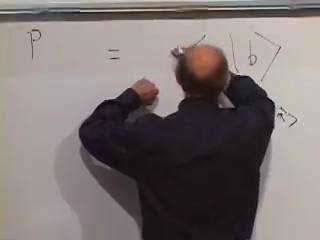
\includegraphics[width=0.78\linewidth]{lecture_03_figure_06.png}
\caption{概率规则被写成重叠与其共轭的乘积。}
\lectureframe{01:16:40}
\end{figure}

\begin{classroomqa}
\lecturetimestamp{01:19:19}
\audiencequestion{这是两个态之间夹角的余弦平方吗？}
\lecturerresponse{对于普通欧几里得空间中的实单位向量，内积就是某个夹角的余弦。而在这里，内积一般是复数，因此并不存在一个普通空间中的夹角使其余弦等于它。有用的类比对象是重叠的模，而概率则是它的绝对平方。}
\end{classroomqa}

\begin{classroomqa}
\lecturetimestamp{01:20:18}
\audiencequestion{如果制备态是\(M\)的另一个具有不同本征值的本征向量，那会怎样？}
\lecturerresponse{那么这两个本征向量正交。它们的重叠为零，因此得到\(\lambda_A\)的概率为零。制备一个具有某一确定值的态，就排除了同一可观测量的另一个不同确定值。}
\end{classroomqa}

\begin{classroomqa}
\lecturetimestamp{01:21:23}
\audiencequestion{同一条规则能否处理没有任何结果确定的那种制备？}
\lecturerresponse{能。这正是普遍情形：\(\ket B\)不必是\(M\)的本征态。它与各归一化本征向量的重叠给出相应结果的概率。我们先从一个双结果例子开始，然后再处理更复杂的分布。}
\end{classroomqa}

本讲通过若干制备情形来训练这条规则，而不是把它藏在一个公式里。

首先制备\(\sigma_3=+1\)：
\begin{equation}
  \ket B=\ket{u}=\begin{pmatrix}1\\0\end{pmatrix}.
\end{equation}
测量\(\sigma_1\)。对于它的\(+1\)本征向量，
\begin{equation}
  \braket{x+}{u}
  =
  \frac{1}{\sqrt2}
  \begin{pmatrix}1&1\end{pmatrix}
  \begin{pmatrix}1\\0\end{pmatrix}
  =\frac{1}{\sqrt2},
\end{equation}
因此
\begin{equation}
  P(\sigma_1=+1\mid\sigma_3=+1)=\frac12.
\end{equation}
将\(\ket{x+}\)替换为\(\ket{x-}\)得到相同的概率。交换制备与测量也得到二分之一，因为重叠的绝对平方是对称的。

对于一个真正复数的例子，制备\(\ket{x+}\)并测量\(\sigma_2\)。于是
\begin{align}
  \braket{y+}{x+}
  &=
  \frac12
  \begin{pmatrix}1&-i\end{pmatrix}
  \begin{pmatrix}1\\1\end{pmatrix}
  =\frac{1-i}{2},
  \notag\\
  P(\sigma_2=+1\mid\sigma_1=+1)
  &=\left|\frac{1-i}{2}\right|^2
  =\frac14+\frac14
  =\frac12.
  \label{eq:l03-complex-probability-example}
\end{align}
因此，沿一个轴制备自旋并沿垂直轴测量，会给出两个结果的等概率。

\section{指针、态与任意轴}

如果不修正术语，前面这句话可能会被误解。磁矩具有空间方向，我们将其称为\emph{指针}。而ket是复态空间中的向量。两个空间指针可以垂直，而两个态向量可以正交。这些是在不同空间中的不同陈述。

\begin{classroomqa}
\lecturetimestamp{01:29:25}
\audiencequestion{如果两个物理自旋方向相差九十度，它们的态向量应当正交吗？}
\lecturerresponse{不应当。沿垂直空间轴的自旋向上态，其重叠平方为\(1/2\)，而不是零。与沿某一轴的自旋向上态正交的态，是沿同一轴的自旋向下态。我们把\emph{垂直}保留给普通空间中的指针，而把\emph{正交}保留给完全可区分的态。}
\end{classroomqa}

\begin{classroomqa}
\lecturetimestamp{01:31:25}
\audiencequestion{我们能否用\emph{线性无关}来代替\emph{正交}？}
\lecturerresponse{不能。线性无关只是说没有任何向量是其他向量的标量倍；它并不要求内积为零。正交性是更强的条件，并且在这里承载着完全可区分性的物理含义。}
\end{classroomqa}

令\(\hat n=(n_1,n_2,n_3)\)为普通空间中的单位指针：
\begin{equation}
  n_1^2+n_2^2+n_3^2=1.
\end{equation}
沿该方向的自旋算符是点积的矩阵值类比：
\begin{equation}
  \boldsymbol{\sigma}\cdot\hat n
  =
  n_1\sigma_1+n_2\sigma_2+n_3\sigma_3
  =
  \begin{pmatrix}
    n_3&n_1-in_2\\
    n_1+in_2&-n_3
  \end{pmatrix}.
  \label{eq:l03-spin-arbitrary-axis}
\end{equation}
它是厄米的：对角元为实数，非对角元互为共轭。

\begin{figure}[htbp]
\centering
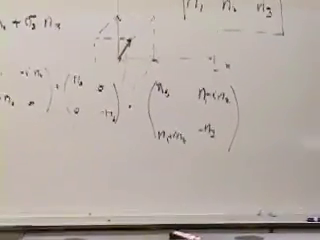
\includegraphics[width=0.84\linewidth]{lecture_03_figure_07.png}
\caption{空间单位指针、算符和式及其显式厄米矩阵被一起展开。}
\lectureframe{01:38:00}
\end{figure}

要找出它可能的值，先将其平方，再代入矩阵元素。矩阵的次序很重要，因此交叉项以反对易子的形式出现：
\begin{align}
  (\boldsymbol{\sigma}\cdot\hat n)^2
  &=
  n_1^2\sigma_1^2+n_2^2\sigma_2^2+n_3^2\sigma_3^2
  \notag\\
  &\quad
  +n_1n_2(\sigma_1\sigma_2+\sigma_2\sigma_1)
  \notag\\
  &\quad
  +n_2n_3(\sigma_2\sigma_3+\sigma_3\sigma_2)
  \notag\\
  &\quad
  +n_1n_3(\sigma_1\sigma_3+\sigma_3\sigma_1).
  \label{eq:l03-axis-square-expanded}
\end{align}
不同的泡利矩阵彼此反对易：
\begin{equation}
  \sigma_i\sigma_j+\sigma_j\sigma_i=0
  \qquad(i\ne j).
  \label{eq:l03-pauli-anticommutation}
\end{equation}
讲义明确检验了其中一个情形：
\begin{equation}
  \sigma_1\sigma_3
  =
  \begin{pmatrix}0&-1\\1&0\end{pmatrix},
  \qquad
  \sigma_3\sigma_1
  =
  \begin{pmatrix}0&1\\-1&0\end{pmatrix}
  =-\sigma_1\sigma_3.
  \label{eq:l03-order-check}
\end{equation}

\begin{figure}[htbp]
\centering
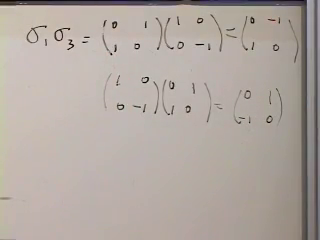
\includegraphics[width=0.82\linewidth]{lecture_03_figure_08.png}
\caption{将\(\sigma_1\)与\(\sigma_3\)按相反次序相乘，所得矩阵相差一个负号。}
\lectureframe{01:44:50}
\end{figure}

式~\eqref{eq:l03-axis-square-expanded}中的交叉项消失，而\(\sigma_i^2=I\)。因此
\begin{equation}
  (\boldsymbol{\sigma}\cdot\hat n)^2
  =(n_1^2+n_2^2+n_3^2)I
  =I.
\end{equation}
于是每个本征值都满足\(\lambda^2=1\)：
\begin{equation}
  \lambda=\pm1.
\end{equation}
无论装置选取哪条空间轴，探测器仍然只有\(+1\)和\(-1\)这两个结果。邻近方向之间的关系并不表现为某个中间测量值，而是体现在这两个固定答案的概率之中。
